\documentclass[11pt,reqno]{amsart}

% ============================================================
%  Math for AI Safety
%  Ported to amsart (mytemplate.tex house style).
%  Citations: numbered \cite with hyperref links; bibliography is a
%  manual thebibliography. arXiv links via the \arxiv macro.
% ============================================================

\usepackage[T1]{fontenc}
\usepackage{amsmath, amssymb, amsthm, mathtools}
\usepackage{graphicx}
\usepackage{enumitem}
\usepackage{array}
\usepackage{longtable}
\usepackage{microtype}
\usepackage[normalem]{ulem} % \uline for glossary terms at first use; normalem keeps \emph italic
\usepackage{tikz}
\usetikzlibrary{arrows.meta, positioning, calc, decorations.pathreplacing, shapes.geometric}
\usepackage[colorlinks=true, linkcolor=blue!55!black, citecolor=blue!55!black, urlcolor=blue!55!black]{hyperref}
\hypersetup{pdftitle={Math for AI Safety: An Invitation for Mathematicians}, pdfauthor={Lionel Levine}}

% Wider text block (mytemplate.tex house style).
\addtolength{\oddsidemargin}{-.2in}
\addtolength{\evensidemargin}{-.2in}
\addtolength{\textwidth}{.4in}

% Clickable arXiv links (from mytemplate.tex).
\newcommand{\arxiv}[1]{\href{http://arxiv.org/abs/#1}{\texttt{arXiv:#1}}}
% Glossary terms are underlined at first use (2026-07-13, per Lionel); the intro says so.
\DeclareRobustCommand{\glsfirst}[2]{\hypertarget{first:#1}{\hyperlink{gloss:#1}{\uline{#2}}}}
\DeclareRobustCommand{\glsentry}[2]{\hypertarget{gloss:#1}{\hyperlink{first:#1}{#2}}}

\theoremstyle{plain}
\newtheorem*{theorem*}{Theorem}
\theoremstyle{definition}
% A small marker for the starred open problems.
\newcommand{\op}{\ensuremath{\bigstar}\;}
\newtheorem{openproblem}{\op Open Problem}

\title[Math for AI Safety]{Math for AI Safety: \\ An invitation for mathematicians}
\author{Lionel Levine}
\date{July 22, 2026}

\begin{document}

\begin{abstract}
Powerful AI systems raise questions that look, at first, like engineering: What should the system optimize? What has it learned? Why does it generalize? How will it behave on unfamiliar inputs? Each has a mathematical core. I organize this invitation by mathematical field, so you can turn straight to your own: logic and game theory for cooperation and bounded reasoning; probability and causality for agency and world-models; algebra and representation theory for learned features; analysis and geometry for generalization and training dynamics. New mathematics is needed to help make AI systems more legible, steerable, and cooperative. Each section ends with a concrete open problem, chosen to be small enough to start and close enough to the safety question to matter.
\end{abstract}

\maketitle

\section{Introduction}
\label{sec:intro}

\subsection{Three kinds of mathematician}

I would like to distinguish three stances a mathematician can take toward the arrival of capable AI. The \emph{artisanal} mathematician does mathematics by and for humans: each theorem, definition, and proof is bespoke, valued for its beauty and for the understanding it produces. Until very recently, all mathematics was artisanal.\footnote{I chose the terms ``artisanal'' and ``industrial'' for their mixed connotations, reflecting real tradeoffs between these two stances. \emph{Artisanal} evokes uniqueness and skilled craft, along with a suggestion of being quaint or old-fashioned. \emph{Industrial} evokes modern efficiency and scale, along with a suggestion of inhumanness or lack of soul. These two terms draw a parallel between mathematics today and the trades that were disrupted by automation during the Industrial Revolution.}
The \emph{industrial} mathematician embraces AI as a collaborator and an accelerant: AI systems take part in proof and discovery~\cite{spherepacking2026,openai2026unitdistance,alon2026remarks,sawin2026}, and the output is often a machine-checkable formal proof~\cite{mathlib2020}.
The \emph{civic} mathematician turns our craft toward a third end: helping humanity steer and adapt to the disruptions caused by our own technologies. The civic stance differs from the traditional stance of an applied mathematician in its big-picture viewpoint: the civic mathematician recognizes that solving any particular engineering challenge may or may not benefit humanity, and seeks out the challenges with the potential for the most benefit.\footnote{I chose the term ``civic'' to emphasize that steering our technology is a team effort, arising from a sense of duty to community, including large-scale communities like humanity and the planet.}

These three stances classify mathematicians by how they relate to AI; in contrast, Gowers (theory builders/ problem solvers~\cite{gowers2000}) and Dyson (birds / frogs~\cite{dyson2009}) classify mathematicians by how they relate to mathematics itself. 
The stances are not exclusive: one can prove a theorem for its intrinsic beauty, and also formalize the proof, and also ask what it implies for AI safety. But the civic stance invites a new perspective on an old question: of all the theorems we might prove, which ones deserve the effort?  This survey is an invitation to try the civic stance.

\subsection{What is our profession's purpose?}

Thurston asked a version of this question in ``On proof and progress in mathematics,'' and answered that what mathematicians accomplish is to advance human understanding of mathematics~\cite{thurston1994}. That understanding does not stay within the profession. Mathematics is one of the ways society builds its future. Our students become AI engineers, our theorems become tools in their hands, and our definitions become the language they use to describe what they are building.

%Technological progress emerges from choices made by human researchers and engineers. 
Already we defer to systems we do not fully understand. Among the many risks from developing powerful AI systems, one of the most alarming is \glsfirst{gradual-disempowerment}{gradual disempowerment}~\cite{kulveit2025}. The mechanism has two parts. First, competitive pressure drives delegation to technology we do not understand: a trading bot outperforms a human trader, though even its creators cannot say what makes it profitable; and those who do not delegate are increasingly outcompeted by those who do. Second, what keeps large institutions approximately aligned to human interests is that, for now, those institutions are made of humans; when companies, nation states, and militaries are made mostly of AI agents, their goals and values may drift away from what humans value. The first part erodes our understanding of the world, and hence our power over it; it also sets the stage for the second.

Preventing AI harms is in part a \emph{mathematical} problem, and the purpose of this survey is to recruit mathematicians to work on it. Only in part: what AI ought to do, and who decides, are questions of philosophy, ethics, economics, and politics. This survey keeps to the mathematical part of a much larger conversation.

\subsection{Where mathematicians plug in}
\label{sec:pipeline}

At a high level, an AI system is produced in five stages, beginning with defining the desired behavior and ending with deploying the trained system, after which unanticipated failures feed back into refining the earlier stages (Figure~\ref{fig:pipeline}).

To illustrate the five stages, consider the problem of building a tool for proving inequalities in a proof assistant:

\begin{itemize} 
  \item \emph{Define}: given hypotheses $H$ and a proposed inequality $I$, the system should either produce a formally checkable proof of $H\Rightarrow I$ or say ``unknown.'' 
  \item \emph{Measure}: score the fraction of benchmark statements proved within a fixed time and proof-length budget. 
  \item \emph{Train}: show the system many proof traces, say sums-of-squares certificates, AM--GM arguments, and induction templates. 
  \item \emph{Test}: hold out new inequalities from specified families. 
  \item \emph{Deploy}: let the tool  suggest lemmas inside a mathematician's formalization workflow. 
\end{itemize}

After deployment, the failures come back. It returns a valid proof, but of a statement weaker than intended: a gap in the \emph{definition} of the desired behavior. Its pass rate is high because the benchmark is full of short template problems, while the mathematician needs one nontrivial lemma: a gap in what we \emph{measured}. It is brittle on boundary cases such as equality and zero denominators, which were rare in the proof traces: a gap in what it was \emph{trained} on. And it passes the holdout set because the generator reused the same normal forms and substitutions: a gap in the \emph{test}. Each backward arrow is its own piece of mathematics: formal specification, scoring rules, distribution design, and adversarial test construction.

The inequality example is deliberately mathematical, but the same basic pipeline applies across many areas, whether it is an image classifier for a medical application, a control system for a self-driving car, or a content recommendation system. Machine-learning research often concentrates on the \emph{training} and \emph{testing} stages, while engineers focus on \emph{deployment}. The earlier stages rely on mathematicians, philosophers, economists, and others to supply the \emph{defining} and \emph{measuring} inputs. %The harms of social media are in part due to the failure to define and measure the desired consequences of an AI system.

\begin{figure}[ht]
\centering
\resizebox{0.96\textwidth}{!}{%
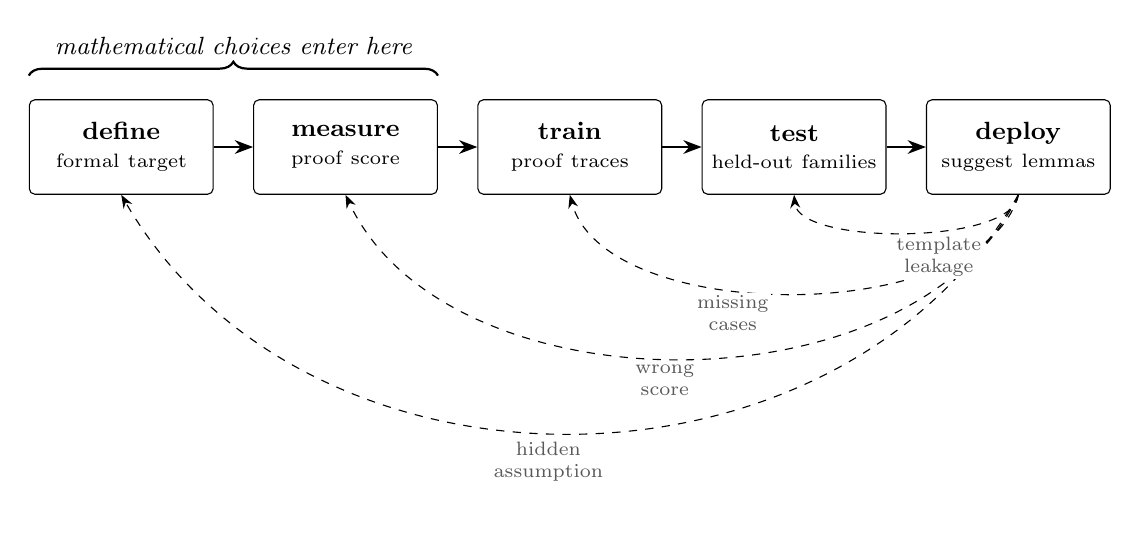
\begin{tikzpicture}[
  >=Stealth,
  box/.style={draw, rounded corners=2pt, minimum height=12mm, text width=21mm, align=center, font=\small},
  lab/.style={font=\scriptsize, align=center, fill=white, inner sep=1pt, text=black!65},
  node distance=8mm and 5mm]
  \node[box] (def)  {\textbf{define}\\[-1pt]\scriptsize formal target};
  \node[box, right=of def]   (meas)  {\textbf{measure}\\[-1pt]\scriptsize proof score};
  \node[box, right=of meas]  (train) {\textbf{train}\\[-1pt]\scriptsize proof traces};
  \node[box, right=of train] (test)  {\textbf{test}\\[-1pt]\scriptsize held-out families};
  \node[box, right=of test]  (dep)   {\textbf{deploy}\\[-1pt]\scriptsize suggest lemmas};
  \draw[->, thick] (def)--(meas); \draw[->, thick] (meas)--(train);
  \draw[->, thick] (train)--(test); \draw[->, thick] (test)--(dep);
  \draw[->, dashed] (dep.south) to[out=-120,in=-60,looseness=1.05]
    node[pos=.52, lab, below=2pt] {hidden\\assumption} (def.south);
  \draw[->, dashed] (dep.south) to[out=-115,in=-65,looseness=.92]
    node[pos=.52, lab, below=1pt] {wrong\\score} (meas.south);
  \draw[->, dashed] (dep.south) to[out=-105,in=-75,looseness=.78]
    node[pos=.6, lab, below=1pt] {missing\\cases} (train.south);
  \draw[->, dashed] (dep.south) to[out=-95,in=-85,looseness=.58]
    node[pos=.4, lab, below=1pt] {template\\leakage} (test.south);
  \draw[decorate, decoration={brace, amplitude=5pt}, thick]
    ($(def.north west)+(0,3mm)$) -- ($(meas.north east)+(0,3mm)$)
    node[midway, above=4pt, font=\small\itshape] {mathematical choices enter here};
\end{tikzpicture}
}
\caption{A schematic pipeline for producing an AI system, illustrated by a tool for proving inequalities. The forward arrows build the system; the dashed arrows represent deployment failures that inform improvements of each stage of the pipeline.}
\label{fig:pipeline}
\end{figure}

% control/coexistence paragraph and its footnote commented out 2026-07-09 (pending a fuller argument for coexistence, perhaps as a separate piece). Companion comments: glossary row for corrigibility and bibitem harms2024 in conclusion.tex.
% AI safety is sometimes posed as \emph{control}---retaining power over systems more capable than ourselves---which looks like a very hard problem. \emph{Coexistence}, a stable and mutually beneficial relationship with systems we do not fully control, is a larger target and thus an easier one to hit; much of the mathematics below is best read as aiming for coexistence rather than control.\footnote{This goal is contested. Many find it alarming to aim for any future where humans are not in control, and some cannot imagine coexistence without control; Harms~\cite{harms2024}, for example, argues for building AI systems whose overriding goal is \glsfirst{corrigibility}{corrigibility}, remaining correctable by their human principals. The case for coexistence deserves a fuller argument than I can make here.}

This invitation is organized by mathematical field, so you can turn directly to yours. Each section states the safety stakes, narrates at least one theorem, and ends with at least one open problem (\ensuremath{\bigstar}). Each open problem has a detailed companion: a self-contained supplement that fixes every definition, states each question precisely, and records what is already settled, available at \url{https://lionellevine.github.io/MAIS/open-problems}. % \op includes a trailing \; for theorem headers; use the bare star in parentheses
I keep machine-learning jargon to a minimum; a short glossary appears in Appendix~\ref{app:glossary}, and each glossary term is underlined at its first appearance.

\section{Logic and game theory: when do AI agents cooperate?}
\label{sec:logic}

Two programs that can read each other's source code can be made to cooperate in a one-shot Prisoner's Dilemma---provably, and (under explicit assumptions about the proof system) unexploitably, without checking that they are copies of one another. Behind this surprise is L\"ob's theorem, a corner of mathematical logic rarely introduced through applications.

\subsection{The game changes when the players can read each other}

The Prisoner's Dilemma is the standard model of a cooperation failure: each player does better by defecting whatever the other does, yet mutual cooperation $(C,C)$ beats mutual defection $(D,D)$. In the usual one-shot game, defection is dominant. But that analysis assumes the players are \emph{opaque} to each other. When two agents are programs, each can be handed the other's source code before choosing its action. This is the setting of \emph{open-source game theory}, or \emph{program games}, studied since Howard~\cite{howard1988} and Tennenholtz~\cite{tennenholtz2004}.

One idea already breaks the classical verdict. Let $\mathrm{CliqueBot}$ be the program ``cooperate if and only if the opponent's source code is byte-for-byte identical to mine.'' Two CliqueBots cooperate, and CliqueBot is never exploited (it never cooperates with an opponent that defects against it), so $(C,C)$ is reachable and stable. But CliqueBot is a poor citizen: it refuses to cooperate with an agent that is functionally identical yet formatted differently, or written in another language. We want cooperation that is \emph{robust}---keyed to what the opponent \emph{does}, not to the syntax of how it is written.

\subsection{FairBot and the L\"obian argument}

Consider instead $\mathrm{FairBot}$: \emph{cooperate if and only if you can prove (in Peano Arithmetic, say) that the opponent cooperates with you.} Two FairBots reason about each other's behavior, not each other's syntax. Naively this looks like an infinite regress---each waits to prove something about the other, who is waiting in turn---and almost every mathematician, asked to guess, predicts mutual defection. The guess is wrong.

\begin{theorem*}[Bar\'asz, Christiano, Fallenstein, Herreshoff, LaVictoire, Yudkowsky~\cite{barasz2014}]
FairBot cooperates with itself: $\mathrm{PA} \vdash [\,\mathrm{FairBot}(\mathrm{FairBot}) = C\,]$. Moreover FairBot is \emph{unexploitable}: assuming PA proves only true facts about the outputs of the programs in question, FairBot never cooperates with an opponent that defects against it.
\end{theorem*}

(Here $\mathrm{PA}\vdash\varphi$ means that the sentence $\varphi$ is provable in Peano Arithmetic.) The proof is a simple application of L\"ob's theorem, a strengthening of the self-reference behind G\"odel's second incompleteness theorem.\footnote{In the special case $\varphi=\bot$, L\"ob's theorem says that if PA proves its own consistency then PA proves a contradiction---G\"odel's second incompleteness theorem.} Write $\Box\varphi$ for the arithmetical sentence $\mathrm{Prov}_{\mathrm{PA}}(\ulcorner\varphi\urcorner)$, read as ``$\varphi$ is provable in PA.''

\begin{theorem*}[L\"ob~\cite{lob1955}]
For any sentence $\varphi$, if $\mathrm{PA} \vdash (\Box \varphi \to \varphi)$ then $\mathrm{PA} \vdash \varphi$.
\end{theorem*}

Let $\varphi$ be the sentence ``both FairBots cooperate.'' Each FairBot cooperates exactly when it finds a proof that the other does; so \emph{if it is provable that both cooperate, then both genuinely do}---that is, $\mathrm{PA} \vdash (\Box\varphi \to \varphi)$. L\"ob's theorem now delivers $\mathrm{PA} \vdash \varphi$ outright, and both cooperate!

FairBot as stated searches proofs of unbounded length. Critch~\cite{critch2016} supplies a computable version, $\mathrm{FairBot}_k$, that searches only proofs of length at most $k$ (write $\Box_k\varphi$ for ``$\varphi$ has a proof of length $\le k$''), and shows that, for proof systems able to certify the cost of recognizing their own bounded proofs (a hypothesis the supplement to the open problem below examines closely), it still cooperates with itself once $k$ is large enough---turning the L\"obian argument into a terminating computation and making the question quantitative: how large must $k$ be?

A third family of strategies, after the identity-based CliqueBot and the L\"obian FairBot, is \emph{simulation-based}: instead of searching for a proof that the opponent cooperates, run the opponent's code and do what it does, cooperating outright with some small probability so that mutual simulation terminates. Cooper, Oesterheld, and Conitzer~\cite{cooper2025} characterize the equilibria such strategies achieve; proponents argue that simulation is more robust, and less mind-bending, than the L\"obian approach.

\subsection{Why a safety researcher cares---and worries}

The FairBot theorem is a proof of concept: given enough mutual transparency, agents can cooperate where classical game theory predicts defection. Humans approximate this transparency only at great cost, in contracts, treaties, and audits, to make their commitments credible~\cite{schelling1960}. For programs, half of transparency is free: handing over source code costs nothing. Making sense of the code one receives is the expensive half; for agents built on \glsfirst{neural-network}{neural networks}, it is the interpretability problem of Section~\ref{sec:interp}. Still, AI agents are programs, and as they begin to transact with one another, the program game becomes a natural model of their dealings---with the cost of cooperation set by the cost of verification, the subject of the open problem below.

The same transparency is also a hazard: mutually transparent agents can reach cooperative equilibria---including collusion \emph{against} their human principals---that humans can neither match nor detect. And the map from transparency regime to outcome is full of surprises: Critch, Dennis, and Russell~\cite{critch2022} exhibit natural institution designs whose large-resource behavior is the opposite of what one first expects. Nearly all of this design space is unexplored; the same paper collects open problems in it, including specific matchups whose outcomes are conjectured but unproved. The \emph{safe Pareto improvements} of Oesterheld and Conitzer~\cite{oesterheld2021}---commitments guaranteed to leave every principal at least as well off---pose more.

Logical induction~\cite{garrabrant2016} is the probabilistic companion to this bounded-proof story. A \emph{logical inductor} assigns prices $\mathbb{P}_n(\varphi)$ to arithmetical sentences on day $n$, as if each sentence were a stock, while a slow deductive process reveals more theorems. The criterion is a bounded Dutch-book condition: no polynomial-time trader with bounded risk may make unbounded profit by buying and selling these sentence stocks. It answers, with a theorem, the question this survey began with: how should a reasoner with finite computation allocate probability mass over facts it has not yet proved?

\subsection{Open problems}

\begin{openproblem}[Quantitative bounded L\"ob]
Fix a proof system $S$, a G\"odel coding, and the provability predicate $\Box^S$; write $S\vdash_{\le k}Q$ for an $S$-proof of $Q$ of at most $k$ symbols. Determine the least overhead $F_S$ for which
\[
   S\vdash_{\le k}(\Box^S P\to P)
   \quad\text{implies}\quad
   S\vdash_{\le F_S(k,|P|)} P,
\]
where $|P|$ is the length of the sentence $P$: given a $k$-symbol proof of the hypothesis of L\"ob's theorem, how many symbols can the shortest proof of its conclusion require? A polynomial upper bound for one standard system, with explicit constants, would turn the L\"obian argument from a possibility theorem into a budget. The first instance with a game attached: Critch's theorem~\cite{critch2016} gives a finite threshold $\hat k$ above which two copies of $\mathrm{FairBot}_k$ provably cooperate, assuming the proof system can certify the cost of noticing its own bounded proofs; verify that hypothesis, with constants, for a specific system and coding. A first computation, before any asymptotics: implement bounded proof search in a weak system for two explicitly supplied agents, and tabulate the smallest $k$ at which cooperation appears. Over a family of such agent pairs, does $\hat k$ grow polynomially in the agents' description length?
\end{openproblem}

% \noindent\emph{Entry points.} Provability logic (G\"odel--L\"ob, $\mathsf{GL}$) and modal fixed points; proof complexity (for the bounded theory); computational game theory and mechanism design; decision theory; logical uncertainty.

\section{Probability and causality: what is an agent?}
\label{sec:epistemics}

% Section opening restructured 2026-07-13 per Lionel: agentic rise -> counteract the
% "only the operator has a goal" reflex -> safety depends on goals AND beliefs (drone)
% -> degrees of agency (thermostat/chess/human) + METR time horizon -> observational
% vs. intrinsic -> the two pictures, now in separate subsections.
AI systems are becoming \emph{agentic}: able to operate independently in pursuit of a goal. The first chat assistants answered the question put to them and stopped; their successors browse the web, write and run code, and carry out multi-day projects. Agency is useful, and the market is supplying it.

An old reflex objects: software cannot have goals---the goal belongs to the operator, and the software only transmits it. For calculators and compilers the reflex is right. But nobody writes the rule a trained agent follows---it is grown, not specified---and when such an agent books a wrong flight, even its operator asks what it was \emph{trying} to do. The reflex deserves an answer, not a dismissal: a definition of \emph{goal} precise enough to settle whether a trained network has one.

The definition matters for safety, because whether an agent is safe depends in part on its goals and its beliefs. Goals first: the same drone can deliver a pizza to your house or a bomb. But a friendly goal is not enough, because even the pizza drone is unsafe if its beliefs are false: a drone whose map labels the freeway shoulder as your street will set dinner down in traffic.

Agency also comes in degrees. A thermostat pursues a temperature; a chess engine pursues checkmate, planning many moves ahead; a human being chooses their goals, revises them, and pursues them for decades. What exactly increases along this scale? Pending a definition, one can still measure: the \emph{time horizon} of an AI system is the length of task---measured by the time it takes a skilled human---that the system can complete at least half the time. Across systems released since 2019, the time horizon has doubled roughly every seven months, from seconds to about an hour~\cite{kwa2025}.

The time horizon is an observational measure: it tracks agency by watching behavior on benchmark tasks, without saying what a goal or a belief \emph{is}. The early stages of the pipeline of Section~\ref{sec:pipeline}---\emph{define} and \emph{measure}---ask for more: mathematical definitions of these words, intrinsic to the agent. Probability supplies two candidate pictures: an agent as something that maximizes expected utility, and an agent as something that keeps a probabilistic model of the hidden states behind its observations. Causality then asks when such a world-model can be recovered from behavior. Beliefs answer to what is true, goals to what is good; one would expect belief update and action choice to be governed by different mathematics.

\subsection{The agent as utility maximizer}

The \emph{utility maximizer} has a current belief $q(z)$ over possible states $z$ of the world and a utility function $u(\tau)$ assigning a number to each full outcome or trajectory $\tau$. In a sequential setting, an ``action'' is a \glsfirst{policy}{policy} $\pi(a\mid h)$: a rule, possibly stochastic, for choosing an action $a$ from the information history $h$ available so far. Thus $h$ is the observed past, $\tau$ the whole course of events including the future; the belief $q$ and the agent's \emph{world-model}---its model of how actions affect the world---combine with $\pi$ to induce a probability measure $Q_\pi$ on trajectories, and the agent chooses $\pi$ to maximize expected utility $\mathbb{E}_{\tau\sim Q_\pi}[u(\tau)]$.

Von Neumann--Morgenstern~\cite{vnm1944} gives the classical representation theorem. A \emph{lottery} is a probability distribution over outcomes, and an agent's \emph{preferences over lotteries} are its rankings of these distributions: gambles, not just sure things. If the rankings satisfy a small list of consistency axioms---completeness (any two lotteries can be ranked), transitivity, continuity, and independence (mixing both lotteries with a common third, in the same proportion, does not change their order)---then the agent behaves as if maximizing expected utility, with $u$ unique up to positive affine transformation.

If several systems are competing for the same resources, and one of them has cyclic or otherwise exploitable preferences, then a competitor whose preferences satisfy the axioms---equivalently, one that maximizes some expected utility---will tend to beat it. (An agent with cyclic preferences will pay to trade its way around the cycle, ending where it began.) Over time, this creates a selection pressure toward agents that are well modelled as maximizing some objective, even if they were not designed that way. This selection argument is a heuristic, not a theorem, though it has a rigorous kernel, Wald's complete class theorem: under compactness and continuity hypotheses on the decision problem, every \emph{admissible} decision rule---one that no rival improves on everywhere, strictly somewhere---is a Bayes rule for some prior, or a limit of Bayes rules~\cite{wald1950}. The selection argument is a second reason, after market demand, to expect AI systems to grow more agentic.

The von Neumann--Morgenstern theorem comes with a caveat as important as the theorem itself: it assumes that the outcome space and the preferences are already given; it does not tell us what a trained network's outcomes are, what its utility is, or whether its apparent preferences are complete and stable (the same from one context, or one day, to the next).

\subsection{The agent as active predictor}

For a picture that fits trained networks natively, start from what we know with certainty: the training objective. A \glsfirst{language-model}{language model} is a neural network trained to predict the next word-fragment of text. Its objective is its mean \emph{surprise}: the average, over an enormous corpus of human writing, of minus the logarithm of the probability it assigned to the fragment that actually came next. Whatever later training makes of it, a language model is by construction a predictor---suggesting a theory of agency that takes prediction, not preference, as primitive.

The \emph{active predictor} is a picture rooted in models of perception~\cite{rao1999}. Write $z$ for the relevant state of the world and $x$ for the present observation---say, the pixels arriving at the retina. A generative model is a joint density $p(x,z)$, read as ``states $z$ generate observations $x$.'' This $p$ is the agent's standing world-model. (A two-state example to carry along: $z\in\{\text{rain},\text{sun}\}$, $x\in\{\text{wet pavement},\text{dry pavement}\}$, and $p$ makes sun-with-wet an unlikely pair.) The agent also maintains a distribution $q(z)$, its current belief about the hidden state, which it updates on receiving a new observation $x$. In practice $q$ is usually restricted to a simple family $\mathcal Q$, and the agent tries to make $q$ close to the exact posterior $p(z\mid x)$ implied by its world-model.

Here ``close'' is measured by \emph{Kullback--Leibler divergence}. For probability densities $r$ and $s$ on the same space,
\[
   \mathrm{KL}(r\|s)=\int r(z)\log\frac{r(z)}{s(z)}\,dz.
\]
Gibbs' inequality says $\mathrm{KL}(r\|s)\ge0$, with equality if and only if $r=s$ almost everywhere. In information-theoretic terms, $\mathrm{KL}(r\|s)$ is the mean excess surprise of an observer who sees a sample drawn from $r$ but believes the sample was drawn from $s$. It is not symmetric, so it is not a metric; it is a directed measure of how badly $s$ approximates $r$.

Multiplying per-fragment probabilities, a language model also assigns a probability $s(x)$ to each whole text $x$, defining a distribution $s$ over texts. Its training minimizes an empirical estimate of the average surprise $\mathbb{E}_{x\sim r}[-\log s(x)]$, where $r$ is the true distribution of human writing---which equals $\mathrm{KL}(r\|s)$ plus a constant the model cannot affect, the entropy of human writing itself. To train a language model is to drive a KL divergence toward zero.\footnote{When a language model is further trained to maximize a \emph{reward signal} (a numerical score on its outputs that the training pushes up), the standard precaution against \glsfirst{reward-hacking}{reward hacking} (raising the reward in ways that defeat its intent) is a penalty on the KL divergence of the retrained model from the original.}

The active predictor uses the same divergence through the \emph{variational free energy}
\[
   F(q,x)=\mathbb{E}_{q}\!\left[\log q(z)-\log p(x,z)\right]
   =\mathrm{KL}\!\left(q(z)\,\big\|\,p(z\mid x)\right)-\log p(x).
\]
Since KL is nonnegative, this identity shows that $F(q,x)$ is an upper bound on the model's surprise $-\log p(x)$ at seeing $x$. The surprise term does not depend on $q$. Thus, for fixed $x$, lowering $F(q,x)$ lowers this upper bound and makes $q$ a better approximation to the posterior. (In the two-state example: on seeing wet pavement, minimizing $F$ over $q$ moves the belief to the exact posterior---mostly rain.)

\emph{Active inference}~\cite{parr2022} extends the predictor from perception to action. Perception minimizes $F(q,x)$ over beliefs $q$ for fixed observation $x$. Action chooses a policy: each candidate $\pi$ induces the trajectory measure $Q_\pi$ of the utility view, and the agent selects a policy whose predicted futures carry low free energy. The two scores differ in kind: the variational free energy $F$ judges a belief against a present observation, while a policy is judged on observations it has yet to bring about. The simplest such score, the one in Table~\ref{tab:twoviews}, is the total free energy of the predicted trajectory; the \emph{expected free energy} of the active-inference literature refines it, combining preference satisfaction with expected information gain, in forms that vary across that literature. Throughout, one unification holds: the information update and the decision rule---one answerable to truth, the other to goodness---both minimize a free energy built on surprise. Perception lowers free energy by changing the belief to fit the world; action, by changing the world to fit the belief.

% Table restored verbatim from the submitted version 2026-07-16 per Lionel (parallelism
% deliberate), first column unbolded. 2026-07-17 (Sol's final-review item 4): the prose
% now presents the cell as the simplest trajectory score, with the literature's expected
% free energy as its refinement, rather than calling the cell a form of EFE.
\begin{table}[ht]
\centering
\small
\renewcommand{\arraystretch}{1.3}
\setlength{\tabcolsep}{4pt}
\begin{tabular}{@{}>{\raggedright\arraybackslash}p{0.17\textwidth}>{\raggedright\arraybackslash}p{0.39\textwidth}>{\raggedright\arraybackslash}p{0.39\textwidth}@{}}
& \textbf{Agent as utility maximizer} & \textbf{Agent as active predictor}\\
\hline
Core object & World-model $p(x,z)$ and utility $u(\tau)$ & World-model $p(x,z)$ and variational family $\mathcal Q$\\
\hline
Belief update & Bayes: $q_{\rm new}(z)\propto p(x\mid z)q_{\rm old}(z)$ & Variational Bayes: $q_{\rm new}\in\arg\min_{q\in\mathcal Q}F(q,x)$\\
\hline
Policy choice & $\pi^*\in\arg\max_\pi \mathbb{E}_{\tau\sim Q_\pi}[u(\tau)]$ & $\pi^*\in\arg\min_\pi \mathbb{E}_{\tau\sim Q_\pi}\!\left[\sum_t F(q_t,x_t)\right]$\\
\hline
Notation & \multicolumn{2}{>{\centering\arraybackslash}p{0.78\textwidth}@{}}{\shortstack[c]{$z$: state\\
$x$: observation\\
$p(x,z)$: world-model\\
$q(z)$: belief\\
$\tau$: trajectory\\
$\pi$: policy}}\\
\hline
\end{tabular}
\caption{Two views of agency. The utility view starts with preferences, represents them by a utility function $u$, and asks which policy maximizes expected utility over the trajectories it may bring about. This is the natural language for proxy objectives and their failures---optimizing a measurable proxy until it diverges from the goal it stood for (Goodhart's law, reward hacking). The active-predictor view starts with a world-model $p(x,z)$: the agent maintains an approximate belief $q$ in an allowed family $\mathcal Q$, updates $q$ by minimizing variational free energy, and chooses among policies by the free energy of their predicted futures. Here apparent goals can live as priors over observations, so the safety question becomes: what world-model, priors, and inference procedure has the system learned?}
\label{tab:twoviews}
\end{table}

Where in this picture is the goal? Preferences enter as priors over observations: outcomes the agent expects, and therefore acts to bring about. A creature whose model insists that its body temperature is $37^\circ$C registers cold as surprise, and puts on a coat: a goal is a prediction the agent works to make true. Hasn't the theory just conflated false belief with desire? Yes---deliberately: a mistaken prediction is one the agent corrects; a goal is one it keeps. Active inference is thus a candidate \emph{descriptive} theory of agency: a way to recognize beliefs and goals in systems that were never handed a utility function. Ngo's scale-free framing pushes the ambition further: the same analysis might apply to whole agents, to learned personas, or to subagent-like structures inside a network~\cite{ngo2025scale}.


The two views locate the goal differently: written by hand as $u$, or grown inside a learned world-model as a prior. On either view, the world-model is hidden from us. Can behavior reveal it? For agents robust enough, the theorem of the next subsection says it must.

\subsection{Robustness reveals causal structure}

A \emph{Bayesian network} is a directed acyclic graph $G$ whose vertices are random variables $X_1,\dots,X_n$, together with conditional probability tables satisfying
\[
   p(x_1,\dots,x_n)=\prod_i p\!\left(x_i\mid \mathrm{pa}(x_i)\right),
\]
where $\mathrm{pa}(x_i)$ denotes the parents of $X_i$ in $G$. The graph is a bookkeeping device for conditional independence: once the parents of a node are known, its non-descendants add no further information. Pearl's graphical criterion, \emph{$d$-separation}, reads off from the graph exactly which conditional independences are forced by this factorization~\cite{pearl2009}.

A \emph{causal} Bayesian network adds an interpretation to the arrows: each conditional distribution is a local mechanism. An intervention on a variable replaces its usual mechanism by a chosen value or distribution and leaves the other mechanisms alone. This is what distinguishes causation from correlation. If smoke and fire are correlated, observing smoke changes the probability of fire; intervening to make smoke with a smoke machine need not.

The thermostat that began our scale of agency can now be put to the test. Wire its output to an air conditioner in place of a heater---an intervention replacing one mechanism by another---and it will chill the room it was built to warm: whenever the temperature drops, the thermostat calls for more, driving it lower still. The thermostat pursues its temperature only while the mechanisms around it stay fixed; an agent that kept succeeding across such rewirings would need to track which mechanism does what. The theorem below makes this necessity precise.

Richens and Everitt~\cite{richens2024} make the world-model question precise using a \emph{causal influence diagram}: a causal Bayesian network with extra decision nodes, where a policy chooses actions from observations, and utility nodes, whose values the agent is scored on. The agent is tested not just in one environment but across a family of \emph{local interventions}: each either resets some environment variable independently of its usual causes, or \emph{masks} some of the agent's observations, hiding them from view. Its regret under an intervention is the utility gap between its policy and the best policy for that intervened environment.

% Two-variable warm-up added 2026-07-13 (Codex slope report): let the reader
% conjecture the extraction mechanism before the theorem states it in general.
The smallest case shows how behavior can betray a world-model. An agent chooses one of two treatments, and a hidden binary variable decides which treatment works; the agent is scored on curing the patient. Externally set the hidden variable to $1$ with probability $\alpha$---an intervention---and watch the agent as $\alpha$ varies. An agent playing optimally switches treatments at the threshold $\alpha^\star$ where the two treatments' expected utilities cross, and that indifference equation can be solved for the agent's implicit estimate of a causal effect. The theorem turns this trick into a general extraction.

\begin{theorem*}[Robust agents learn causal world models; Richens and Everitt~\cite{richens2024}]
For almost all causal influence diagrams satisfying their regularity assumptions, any policy with regret at most $\delta$ across all local interventions, maskings included, determines an approximate causal model of the utility-relevant environment, with error bounded by a function $\gamma(\delta)$ satisfying $\gamma(0)=0$ and growing linearly for small $\delta$. In the optimal limit $\delta=0$, the graph and joint distribution over all ancestors of the utility are identified exactly.
\end{theorem*}

The proof is constructive: it is the switch-point trick above, repeated. Treating the policy as an oracle, mix interventions pairwise by a parameter $\alpha$ and watch where the optimal action switches; because the utility is known, each indifference equation solves for one interventional probability, and together they recover the conditional distributions and parent sets, except on measure-zero degeneracies such as exact cancellations or ties.

In a follow-up, Richens, Everitt, and Abel~\cite{richens2025general} prove a companion result for goal-directed agents: any agent that generalizes across a large enough family of multi-step goals must have learned a predictive model of its environment, and the model can be extracted from its policy. The more capable the agent, the more accurate the extracted model: for goals that chain $n$ sub-goals in sequence, the error in each extracted transition probability is $O(1/\sqrt{n})$, even for agents that usually fail.

Extraction raises a question of independent interest: the recovered model comes expressed in \emph{some} set of latent variables---whose? If two models predict identically, must their internal variables be translatable into one another, or could an alien mind carve the world into concepts that ours cannot express? Wentworth and Lorell's \emph{natural latents} are a first answer: conditions, robust to approximation, under which the latent variables of two predictively equivalent models must translate into one another's~\cite{wentworth2025}; Eisenstat's \emph{condensation}~\cite{eisenstat2025} approaches the same question from probability, asking how an agent's concepts condense out of its predictive state.

\begin{openproblem}[Behavioral tomography of world-models]
Fix a finite causal influence diagram with binary variables and known utility, and an agent whose policy has regret at most $\delta$ across the family of local interventions. The extraction algorithm behind the theorem above~\cite{richens2024} recovers the agent's causal model from unlimited exact queries to such a policy. Prove a finite-sample version: if each query returns an action sampled from the policy, rather than the policy's exact action probabilities, and each experiment draws on the same intervention family as the theorem, maskings included, how many experiments determine the graph and the conditional probability tables to within $\eta$, and how does the answer scale with $\delta$? As a first case, take the two-variable diagrams, where the \emph{identified set}---the set of models consistent with the agent's observed behavior---can be computed exactly, and measure how the extraction algorithm degrades when its indifference equations are estimated from samples. Interventions on the agent's inputs, or on the \glsfirst{activations}{activations} (the values computed inside its network), are the harder surfaces beyond.
\end{openproblem}

% \noindent\emph{Entry points.} Probability, Bayesian statistics, causal inference, decision theory, identifiability.

% 2026-07-13: \glsfirst anchors moved out of the section/subsection titles (underlined
% glossary links don't belong in headings); the anchors now sit at the first body uses.
\section{Algebra: what is a learned feature?}
\label{sec:interp}

\emph{Mechanistic \glsfirst{interpretability}{interpretability}} tries to reverse-engineer a trained neural network into something a human can read. Much of its core is linear algebra and representation theory: how a network stores more concepts than it has dimensions, and what it means for a concept to be a \emph{direction} one can read or steer.

\subsection{Superposition: packing features into directions}

How does a network with a few hundred dimensions in each layer represent
the many thousands of distinct concepts (``\glsfirst{feature}{features}'')
it seems to know?
A \glsfirst{transformer}{transformer} reads text as a sequence of
\glsfirst{token}{tokens}, words and word-fragments; at any fixed layer,
the computation has the form
\[
\text{text}
\longrightarrow
\text{tokens}
\longrightarrow
\underbrace{(h_1,\ldots,h_T)\in(\mathbb{R}^n)^T}
            _{\text{activations at one layer}}
\longrightarrow
\text{next-token log-probabilities}.
\]
For a text of $T$ tokens, each token position carries a vector
$h_j\in\mathbb{R}^n$.
The copy of $\mathbb{R}^n$ in which these vectors live is the network's
\glsfirst{activation-space}{activation space}.
A leading hypothesis, made vivid by Elhage et al.~\cite{elhage2022},
is \glsfirst{superposition}{superposition}: when features are sparse,
a network can store more of them than it has dimensions, as directions in
activation space that are \emph{not} orthogonal but only nearly so,
tolerating the resulting interference because at any moment only a few
features are active (Figure~\ref{fig:superposition}).
In a small \glsfirst{relu}{ReLU} model one can watch the geometry organize
itself into regular polytopes---antipodal pairs, triangles, pentagons---as
a function of how sparse and how important the features are; it is,
recognizably, a Thomson problem (where do mutually repelling charges
on a sphere come to rest?)~\cite{saff1997}.

\begin{figure}[ht]
\centering
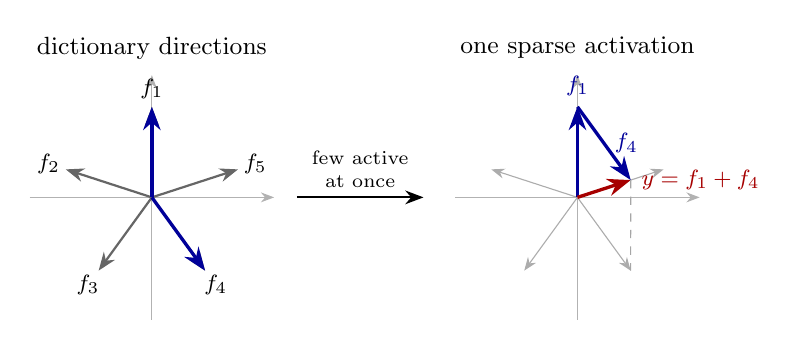
\begin{tikzpicture}[>=Stealth, scale=1.15]
  \begin{scope}
    \node[font=\small] at (0,1.65) {dictionary directions};
    \draw[->, gray!60] (-1.35,0)--(1.35,0);
    \draw[->, gray!60] (0,-1.35)--(0,1.35);
    \foreach \a/\i in {90/1, 162/2, 234/3, 306/4, 18/5} {
      \draw[->, thick, gray!80!black] (0,0) -- (\a:1);
      \node at (\a:1.2) {\footnotesize $f_{\i}$};
    }
    \draw[->, very thick, blue!60!black] (0,0) -- (90:1);
    \draw[->, very thick, blue!60!black] (0,0) -- (306:1);
  \end{scope}
  \begin{scope}[xshift=4.7cm]
    \node[font=\small] at (0,1.65) {one sparse activation};
    \draw[->, gray!60] (-1.35,0)--(1.35,0);
    \draw[->, gray!60] (0,-1.35)--(0,1.35);
    \foreach \a in {90,162,234,306,18} {
      \draw[->, thin, gray!65] (0,0) -- (\a:1);
    }
    \coordinate (a) at (90:1);
    \coordinate (b) at (306:1);
    \coordinate (sum) at ($(a)+(b)$);
    \draw[->, very thick, blue!60!black] (0,0) -- (a) node[above] {\footnotesize $f_1$};
    \draw[->, very thick, blue!60!black] (a) -- (sum) node[midway, right] {\footnotesize $f_4$};
    \draw[->, very thick, red!65!black] (0,0) -- (sum) node[right] {\footnotesize $y=f_1+f_4$};
    \draw[dashed, gray!70] (sum) -- (b);
  \end{scope}
  \draw[->, thick] (1.6,0) -- (3.0,0)
    node[midway, above, font=\scriptsize, align=center] {few active\\at once};
\end{tikzpicture}
\caption{Superposition: five feature directions packed into a two-dimensional space as a regular pentagon. No two are orthogonal, but if only a few features are active at once, the activation is a sparse sum such as $y=f_1+f_4$ and the active directions can still be recovered despite interference.}
\label{fig:superposition}
\end{figure}

The nearest classical analogue is \emph{compressed sensing}~\cite{candes2006,donoho2006}. Picture the features active on a given input as a sparse vector $x\in\mathbb{R}^m$ (only a few of the $m$ possible features fire at once); the network stores it as $y=\Phi x$ in the $n\ll m$ dimensions of its activation space---a linear \emph{measurement}---and reading a feature back out is the \emph{recovery} of $x$ from $y$. Two classical facts explain how this can work. First, there is room for the directions: for every $\varepsilon\in(0,1)$, the space $\mathbb{R}^n$ contains $e^{\Omega(\varepsilon^2 n)}$ unit vectors whose pairwise inner products are at most $\varepsilon$ in absolute value, so the number of $\varepsilon$-almost-orthogonal directions grows \emph{exponentially} in the dimension (a consequence of the Johnson--Lindenstrauss lemma~\cite{johnson1984}). And second, when only a few of those directions are active at once, the stored signal can be read back out. Say that $\Phi\in\mathbb{R}^{n\times m}$ is \emph{restricted-isometric of order $k$} with distortion $\delta$ if
\[
   (1-\delta)\|x\|^2\le\|\Phi x\|^2\le(1+\delta)\|x\|^2
\]
for every \emph{$k$-sparse} vector $x$, meaning one with at most $k$ nonzero entries.

\begin{theorem*}[Cand\`es~\cite{candes2008}; sharp constant, Cai--Zhang~\cite{caizhang2014}]
If $\Phi$ is restricted-isometric of order $2s$ with distortion $\delta<1/\sqrt{2}$, then every $s$-sparse $x\in\mathbb{R}^m$ is the \emph{unique} minimizer of
\[
   \min_{z}\ \|z\|_1 \quad\text{subject to}\quad \Phi z=\Phi x,
\]
and so is recovered \emph{exactly} by a convex program. A random $\Phi$, say with independent Gaussian entries suitably normalized, has the property with high probability once
\[
   n \;\gtrsim\; s\,\log(m/s).
\]
\end{theorem*}

\noindent That last scaling is the quantitative heart of the analogy: the dimension a network needs grows linearly with the number of features active \emph{at once}, and only logarithmically with the total number it can represent. A few hundred dimensions can carry many thousands of features, provided only a handful fire on any given input. For trained transformers this remains an analogy rather than a theorem; turning it into one is part of the invitation.

There is a catch.
Compressed sensing assumes the dictionary $\Phi$ is \emph{known}.
What if someone hands you a trained network and asks what features it
represents?
You can run inputs through the network and record activation vectors,
but the feature directions were not supplied with the
\glsfirst{weights}{weights} (the network's trained parameters).
Recovering the features is therefore a problem in \emph{dictionary learning}:
from the observed activation vectors alone, simultaneously infer a dictionary
$\Phi$ whose columns are feature directions and, for each activation $y$,
a sparse coefficient vector $x$ with $y\approx\Phi x$.
Both the dictionary $\Phi$ and the codes $x$ are unknown.

A \glsfirst{sparse-autoencoder}{sparse autoencoder} attempts this empirically.
It is trained to reconstruct activation vectors using a learned dictionary,
with an $\ell^1$ penalty encouraging each reconstruction to use only a few
dictionary directions.
The resulting directions are often more interpretable than the network's raw
neurons~\cite{bricken2023,cunningham2023}.
This raises an identifiability question: when does the sparse autoencoder
recover features already used by the network, rather than impose a new
coordinate system that merely makes the activations easier to describe?
Classical dictionary learning answers this question when the codes are
exactly sparse and their supports well spread: the dictionary is then
determined up to relabeling and rescaling of its
columns~\cite{aharon2006,hillar2015}, stably in the presence of
noise~\cite{gribonval2015,garfinkle2019}.
Network activations flout these hypotheses because their features co-occur,
which is where the first open problem below begins.

\subsection{Reading, steering, and learned representations}

What could it mean for a concept to be a direction in activation space?
Consider incomplete sentences such as ``The keys on the table \ldots'' and
pause the computation at the activation $h_T$ of the last token.
A linear functional $\ell$ \emph{reads} grammatical number if, for some
threshold $c$, the inequality $\ell(h_T)>c$ predicts that the subject is
plural.
A vector $v\in\mathbb{R}^n$ \emph{steers} toward the plural if replacing
$h_T$ by $h_T+v$ raises the log-probability of ``are'' relative to ``is.''
Thus the same example produces a readout covector $\ell$ and a steering
vector $v$.
Relating them requires an inner product.

Park, Choe, and Veitch~\cite{park2023} formalize these two experiments for
next-token prediction.
They ask whether activation space carries a \emph{causal inner product}
in which independently varying concepts are orthogonal and whose Riesz map
sends readout covectors to steering vectors.
They estimate this geometry from the unembedding matrix
(the model's final linear map, from activation space to next-token
scores).

Arditi et al.~\cite{arditi2024} show that in several open chat models, refusal is mediated by a single direction in the \glsfirst{residual-stream}{residual stream} (the running activation vector that a transformer's layers read from and write to): this direction both predicts whether the model will refuse and causally controls refusal when added or removed. A lone direction serving as both readout and control is evidence for the linear representation hypothesis, though in a different representation space from the unembedding geometry above.

Refusal and its cousins are semantic properties, with no ground truth for what the network \emph{should} compute. Arithmetic is a cleaner laboratory: train a network on a group operation, and the algorithm it ought to discover is known in advance. Representation theory appears in trained arithmetic circuits. A one-layer transformer trained to add integers modulo $p$ learns a discrete-Fourier ``clock'' algorithm, with the characters of $\mathbb{Z}/p\mathbb{Z}$ appearing in its weights~\cite{nanda2023}. Chughtai, Chan, and Nanda~\cite{chughtai2023} take the first step beyond this abelian case. The ambient structure is the Artin--Wedderburn decomposition of the group algebra into matrix blocks,
\[
   \mathbb{C}[G]\;\cong\;\bigoplus_{\rho\in\widehat{G}} M_{d_\rho}(\mathbb{C}),
   \qquad \sum_{\rho\in\widehat{G}} d_\rho^{2}=\lvert G\rvert,
\]
one block per irreducible representation $\rho$. For a nonabelian group the higher-dimensional blocks are genuine matrix representations, and trained networks compute the product through a sparse subset of them. The algorithm's correctness is a representation-theory theorem; that networks implement it is empirical. Which irreducible representations training selects is still something we discover after the fact.

Sometimes the emergence of this structure is a theorem rather than an observation. Marchetti et al.~\cite{marchetti2024} prove that for architectures whose weights are pinned down by the function they compute (up to a unitary change of basis in each unit), invariance under a finite group $G$ forces each unit's weights to be an irreducible unitary representation of $G$; when the weights are moreover orthonormal, together they form the Fourier transform on $G$, and the group itself can be read off the trained weights.

What makes this a safety topic is \emph{selection}: a trained network can discover a crisp algebraic algorithm, hide it in weights, and use only part of the mathematically available structure. If we want to predict a system's behavior off-distribution, it matters which algorithm training found, not only that the training \glsfirst{loss}{loss} is low.

One caveat carries across this whole enterprise: a direction that \emph{predicts} a feature is only a \emph{correlate}. Showing that the network actually \emph{uses} it takes an intervention---ablating the direction, or patching it to the value it would take on another input, and watching the behavior change---not a \glsfirst{probe}{probe} that merely reads it off.

\subsection{Open problems}

% pass 2: moved here from the end of the section, so the section ends on the last open problem rather than on a bibliography pointer
\noindent A broad, structured catalogue of open problems in this area---several with a precise mathematical core---is collected by Sharkey et al.~\cite{sharkey2025}.

\begin{openproblem}[The geometry and identifiability of superposition]
Suppose activations have the form $y=\Phi x+\xi$, where the columns $v_1,\dots,v_m$ of $\Phi$ are unit feature directions, $\xi$ is noise, and the sparse codes $x$ have correlated supports. Estimate the dictionary the way a sparse autoencoder does: minimize reconstruction error plus an $\ell^1$ penalty. Determine, in terms of the coherence $\mu=\max_{i\neq j}\lvert\langle v_i,v_j\rangle\rvert$, the sparsity, the sample size, and the support correlations, when every minimizer recovers the true directions up to permutation and scaling, and when it instead \emph{merges} co-occurring directions into one. Already for two features the answer is unknown: a nested two-event model provably forces merging for every sufficiently small positive penalty, while solo firing restores recovery in the zero-penalty constrained limit; locating the positive-penalty phase boundary is the place to start.
\end{openproblem}

\begin{openproblem}[Training for interpretability]
Post-hoc interpretability asks whether a trained network's features can be recovered after the fact. A complementary problem is to train networks whose features are easier to recover in the first place. In the ReLU toy model of Elhage et al.~\cite{elhage2022} the features are known by construction, so the trade-off can be made exact. Determine the interference--performance frontier: for features appearing sparsely and independently, among weight matrices whose coherence (worst-case interference between stored features) is at most $\mu$, how small can the task loss be, as a function of $\mu$, the sparsity, the number of features, and the number of neurons? A first case: prove or refute that penalizing the \emph{average} interference during training lowers the \emph{worst-case} coherence of the minimizer, compared with training on the task loss alone.
\end{openproblem}

\begin{openproblem}[Representation theory of learned circuits]
Networks trained on group multiplication learn representation-theoretic algorithms~\cite{nanda2023,chughtai2023}, but \emph{which} irreducible representations they use varies from one random seed to the next. Fix a finite group $G$, a one-hidden-layer architecture of fixed width, Gaussian initialization, and gradient flow on the cross-entropy loss (the mean negative log-probability assigned to the correct product) with \emph{weight decay}, an added penalty proportional to the squared norm of the weights. The irreducibles visible in the trained network's outputs then form a random subset of $\widehat{G}$; determine its distribution---which irreducibles are learned, with what probability, as a function of the width and the decay strength. The tables of learned representations in~\cite{chughtai2023} are the data such a theorem would have to explain; the smallest case with genuine competition, $G=\mathbb{Z}/5\mathbb{Z}$ at width two, is open already with the decay switched off.
\end{openproblem}

% \noindent\emph{Entry points.} Linear algebra, compressed sensing, harmonic analysis, representation theory, and differential geometry.

\section{Analysis and geometry: which solution does training find?}
\label{sec:analysis}

\subsection{Why trained networks generalize: singular learning theory}

A trained network is a setting of parameters chosen to fit its \emph{training data}---the finite set of examples it was optimized on. The trouble is that a large network has astronomically many settings that fit those examples perfectly, and they disagree wildly everywhere else; the optimizer---\glsfirst{gradient-descent}{gradient descent}, which repeatedly nudges the parameters downhill on the training error---must land on one of them. For safety, the selected solution matters: a network that behaved well while we were watching may behave differently once deployed. So why do the solutions found by training \emph{generalize}---predict well on fresh data from the same source---when so many other data-fitting solutions would not? These networks reach zero error even when the labels are replaced by pure noise, and a two-layer network with only $2n+d$ parameters can fit \emph{any} labeling of $n$ points in $\mathbb{R}^d$ (Zhang et al.~\cite{zhang2017}); the classical bounds that explain generalization by counting parameters say nothing here.

A different and more general answer comes from \emph{singular learning theory}~\cite{watanabe2009}. Realistic models are \emph{singular}: distinct parameters compute the same function, typically in continuous families, so the optimal set is not an isolated point but a positive-dimensional variety---itself typically singular---flat to second order along its own directions (Figure~\ref{fig:singular-geometry}). The classical large-sample asymptotics all assume an isolated, curved optimum; the right replacements come from algebraic geometry. One caveat: the theory is exact for \emph{Bayesian} learning, not directly for stochastic gradient descent (gradient descent driven by noisy, small-batch estimates of the gradient)---bridging the two is the problem \emph{Opposing staircases} below. The two are closer than they appear: Khan and Rue~\cite{khan2023} derive stochastic gradient descent, along with many other optimizers, as approximations of a single Bayesian update rule.

\begin{figure}[ht]
\centering
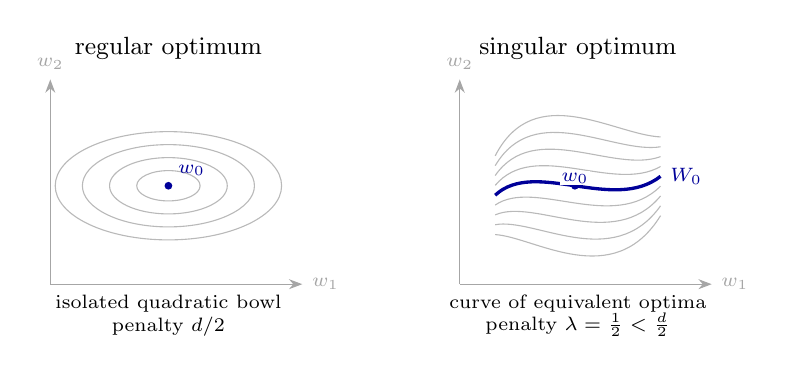
\begin{tikzpicture}[>=Stealth, x=1cm, y=1cm]
  \begin{scope}
    \node[font=\small] at (0,1.75) {regular optimum};
    \draw[->, gray!70] (-1.5,-1.25) -- (1.7,-1.25) node[right, font=\scriptsize] {$w_1$};
    \draw[->, gray!70] (-1.5,-1.25) -- (-1.5,1.35) node[above, font=\scriptsize] {$w_2$};
    \foreach \r in {0.35,0.65,0.95,1.25} {
      \draw[gray!55] (0,0) ellipse ({1.15*\r} and {0.55*\r});
    }
    \fill[blue!60!black] (0,0) circle (1.4pt) node[above right, font=\scriptsize] {$w_0$};
    \node[font=\scriptsize, align=center] at (0,-1.65) {isolated quadratic bowl\\penalty $d/2$};
  \end{scope}
  \begin{scope}[xshift=5.2cm]
    \node[font=\small] at (0,1.75) {singular optimum};
    \draw[->, gray!70] (-1.5,-1.25) -- (1.7,-1.25) node[right, font=\scriptsize] {$w_1$};
    \draw[->, gray!70] (-1.5,-1.25) -- (-1.5,1.35) node[above, font=\scriptsize] {$w_2$};
    \draw[very thick, blue!60!black] (-1.05,-0.12) .. controls (-0.55,0.35) and (0.45,-0.35) .. (1.05,0.12);
    \foreach \s in {0.25,0.5,0.75,1.0} {
      \draw[gray!55] (-1.05,-0.12-\s/2) .. controls (-0.55,0.35-\s) and (0.45,-0.35-\s) .. (1.05,0.12-\s/2);
      \draw[gray!55] (-1.05,-0.12+\s/2) .. controls (-0.55,0.35+\s) and (0.45,-0.35+\s) .. (1.05,0.12+\s/2);
    }
    \fill[blue!60!black] (-0.0375,0) circle (1.4pt)
      node[above, font=\scriptsize, fill=white, inner sep=0.5pt] {$w_0$};
    \node[right, font=\scriptsize, blue!60!black] at (1.05,0.12) {$W_0$};
    \node[font=\scriptsize, align=center] at (0,-1.65) {curve of equivalent optima\\penalty $\lambda=\tfrac12<\tfrac d2$};
  \end{scope}
\end{tikzpicture}
\caption{Regular asymptotics treat the optimum as an isolated quadratic bowl, giving the classical $\tfrac d2\log n$ complexity penalty. Singular learning theory allows a whole variety of parameters to compute the same function: in the right panel the optimal set is a curve $W_0$ through $w_0$, and the penalty $\lambda=\tfrac12$ is strictly smaller than $\tfrac d2=1$, as it is whenever the optimal set has positive dimension.}
\label{fig:singular-geometry}
\end{figure}

% Toy singularity added 2026-07-13 (Codex slope report): one computation the reader
% owns before the formal setup; the exponent/log pair previews (lambda, m).
A toy computation shows what singularity buys. Take first the regular loss $K(w)=w^2$ on the line: the set where $K\le\varepsilon$ is an interval of length $2\sqrt\varepsilon$, so the volume of near-optimal parameters scales as $\varepsilon^{1/2}$---the exponent is $d/2$ with $d=1$. Now take $K(a,b)=a^2b^2$ on the square $[-1,1]^2$. Its zero set is not a point but the union of the two axes, crossing at a singularity, and the region where $K\le\varepsilon$ is a neighborhood of the axes of area of order $\varepsilon^{1/2}\log(1/\varepsilon)$: the exponent stays $1/2$ rather than rising to $d/2=1$, and a logarithm appears. A singular loss has far more near-optimal parameters than its dimension suggests, and the pair (exponent, power of the logarithm) is the simplest instance of the learning coefficient and multiplicity about to be defined.

To make this precise, fix a model $p(x\mid w)$ with parameter $w$ in a compact $W\subseteq\mathbb{R}^d$, a prior $\varphi$ on $W$ (a probability density encoding which parameters are plausible before any data is seen), and a true distribution $q_0(x)=p(x\mid w_0)$ lying in the model. (The subscript keeps the truth $q_0$ apart from the belief $q$ of Section~\ref{sec:epistemics}.) Write
\[
   K(w)=\mathrm{KL}\!\bigl(q_0 \,\big\|\, p(\cdot\mid w)\bigr)=\int q_0(x)\log\frac{q_0(x)}{p(x\mid w)}\,dx ,
\]
the Kullback--Leibler divergence of Section~\ref{sec:epistemics}, so that the set of \emph{true parameters} $W_0=K^{-1}(0)$ is exactly where the model recovers $q_0$.

Given $n$ i.i.d.\ samples $X_1,\dots,X_n$, the central object is the \emph{Bayes free energy}---equivalently the negative log marginal likelihood, the codelength the model assigns to the data,
\[
   \bar F_n \;=\; -\log \int_W \prod_{i=1}^n p(X_i\mid w)\,\varphi(w)\,dw .
\]
(The bar is part of the name; $\bar F_n$ is the random free energy of the sample, not an expectation.) Normalizing the same integrand gives the \emph{posterior} $\propto\prod_i p(X_i\mid w)\,\varphi(w)$---the prior reweighted by how well each parameter fits the data---so $\bar F_n$ is minus the log of its normalizer. This free energy is not the variational free energy $F(q,x)$ of Section~\ref{sec:epistemics}: that one scores a belief against a single observation, this one scores the whole model against a whole sample. The shared name reflects a shared shape, minus the log of a normalizing integral.

Take first the \emph{regular} case: the model is \emph{identifiable} (distinct parameters give distinct distributions) and the optimal set is a single point $W_0=\{w_0\}$ at which the Hessian of $K$---the \emph{Fisher information} $I(w_0)$---is positive-definite. Then the integrand defining $\bar F_n$ concentrates in a shrinking neighborhood of $w_0$; expanding $\log p(X_i\mid w)$ to second order there makes the integral Gaussian, contributing a volume factor $(2\pi/n)^{d/2}\det I(w_0)^{-1/2}$. Taking $-\log$,
\[
   \bar F_n \;=\; nS_n \;+\; \tfrac{d}{2}\log n \;+\; O_p(1),
   \qquad S_n=-\tfrac1n\textstyle\sum_i\log q_0(X_i),
\]
where $S_n$ is the empirical entropy and the remainder is bounded in probability.\footnote{$O_p(1)$ means \emph{bounded in probability}: for every $\varepsilon>0$ there is an $M$ with $\Pr(|\,\cdot\,|>M)<\varepsilon$ for all large $n$.} The complexity penalty is exactly half the parameter count. Watanabe's theorem is the singular replacement, in which $d/2$ gives way to an invariant of the singular geometry.

\begin{theorem*}[Watanabe's free-energy asymptotics~\cite{watanabe2009}]
For a singular model satisfying Watanabe's regularity conditions (real-analyticity and a mild variance bound\footnote{The \emph{relatively finite variance} condition: writing $f(x,w)=\log(q_0(x)/p(x\mid w))$, $K(w)=\mathbb{E}_{q_0} f(X,w)$, and $V(w)=\mathbb{E}_{q_0} f(X,w)^2$, one assumes $V(w)\le C\,K(w)$ near the optimal set---the variance of the log-likelihood ratio is controlled by its mean.}), as $n\to\infty$,
\begin{equation}\label{eq:free-energy}
   \bar F_n \;=\; n\,S_n \;+\; \lambda\log n \;-\; (m-1)\log\log n \;+\; O_p(1),
\end{equation}
where the \emph{learning coefficient} $\lambda>0$---the \emph{real log canonical threshold} (\textup{\textsc{rlct}}) of $K$ relative to the prior $\varphi$---and the integer $m\in\{1,\dots,d\}$, its \emph{multiplicity}, take the places of the $d/2$ and the $1$ of the regular case. The $O_p(1)$ remainder converges in distribution.\footnote{In the regular case the limit is $C-\tfrac12\chi^2_d$ for a constant $C$---the Bayesian shadow of Wilks' theorem, since the log-likelihood-ratio statistic $2\bigl(\sup_w\textstyle\sum_i\log p(X_i\mid w)-\sum_i\log p(X_i\mid w_0)\bigr)\Rightarrow\chi^2_d$. In a singular model the limit is in general non-Gaussian, a functional of a Gaussian process on the manifold obtained by resolving the singularities of $K$.} The same coefficient controls generalization: writing $\hat p_n$ for the posterior average of $p(\cdot\mid w)$, the \emph{generalization error} $G_n=\mathrm{KL}(q_0\,\|\,\hat p_n)$ obeys $\mathbb{E}[G_n]=\lambda/n+o(1/n)$.
\end{theorem*}

The meaning of $\lambda$ is volume growth: the prior volume of the set $\{w\in W : K(w)\le\varepsilon\}$ of parameters fitting the truth to within $\varepsilon$ scales like $\varepsilon^{\lambda}$ times $(\log(1/\varepsilon))^{m-1}$, so smaller $\lambda$ means near-optimal parameters are more plentiful. To compute $\lambda$ for a given model, one resolves the singularities of $K$ (Hironaka~\cite{hironaka1964}).

In the regular case, $\lambda=d/2$ and $m=1$, and the theorem recovers the regular asymptotic expansion above; in a singular model $\lambda\le d/2$, often strictly. The comparison localizes: restrict the integral defining $\bar F_n$ to a neighborhood of one true parameter, and the expansion \eqref{eq:free-energy} holds with that neighborhood's own coefficient. Among the true parameters---all fitting the truth exactly, all weighted by the prior---the posterior share of the most degenerate neighborhoods, those of smallest local $\lambda$, grows with $n$. In this Bayesian setting the posterior concentrates, on its own, on the solutions that the formula $\mathbb{E}[G_n]=\lambda/n$ marks as best-generalizing. This is the theory's rendering of the slogan that learning prefers ``simpler'' solutions: simplicity means a more degenerate geometry, not fewer parameters.

The degeneracy behind a small $\lambda$ is largely \emph{structural}: it comes from directions in parameter space along which the function does not change---for instance those freed when an internal unit is effectively switched off---and these are what pull $\lambda$ below $d/2$. The symmetries are not a defect to be engineered away: within the theory, it is the degeneracy that pulls the generalization error $\lambda/n$ below the classical rate $d/(2n)$.

The coefficient $\lambda$ need not be found by hand. Introduce a knob $\beta>0$, an \emph{inverse temperature}, and the \emph{tempered posterior}
\[
   p_\beta(w)\;\propto\;\varphi(w)\,e^{-\beta n L_n(w)},
   \qquad L_n(w)=-\tfrac1n\textstyle\sum_i\log p(X_i\mid w),
\]
which interpolates between the prior ($\beta=0$) and concentration on the best-fitting parameters ($\beta\to\infty$). (In statistics, taking $\beta<1$ hedges against a misspecified model: Gr\"unwald's ``Safe Bayesian'' learns $\beta$ from the data~\cite{grunwald2012}, and Alquier and Ridgway prove that tempered posteriors still concentrate~\cite{alquier2020}.) At inverse temperature $\beta=1/\log n$, the average of $nL_n$ over the tempered posterior exceeds its minimum by $\lambda\log n$, to leading order~\cite{watanabe2013}. So $\lambda$ can be \emph{estimated} by sampling the tempered posterior, needing neither the true distribution nor an explicit resolution of singularities. That practicality is what lets the theory meet networks far too large to analyze by hand.

What one estimates is not the global $\lambda$ but the \emph{local learning coefficient}: the same invariant computed in a neighborhood of the particular solution $w^\star$ that training actually reached, measuring how degenerate \emph{that} solution is~\cite{lau2023}. As a network trains, its local learning coefficient jumps at discrete moments---\emph{phase transitions}, where the solution moves to a qualitatively new, differently-degenerate part of the landscape as a new piece of internal structure forms. Tracking these jumps is the program of \emph{developmental interpretability}: so far on relatively small networks and with preliminary validation, though the same estimators have already surfaced tens of thousands of candidate structures inside a billion-parameter language model~\cite{murfet2026}.

Two networks can fit the training data identically and yet compute by different internal mechanisms, hence behave differently on inputs outside that data---what ordinary testing, which only probes behavior on data, cannot detect. The singular geometry governs \emph{which} mechanism training selects, and the selection need not favor the mechanisms we would prefer: the most degenerate solution---largest in volume, smallest in $\lambda$---may implement the behavior we intended, or a shortcut that mimics it on the training distribution and fails beyond it. Whether geometric degeneracy favors mechanisms that are also interpretable and robust is, for safety, the question this program must answer; the case that alignment turns on such questions is made in~\cite{lehalleur2025}.

\begin{openproblem}[Does geometric simplicity force a legible mechanism?]
Fix an odd integer $p$ and $H\geq 2p-1$. On input $(a,b)\in(\mathbb{Z}/p\mathbb{Z})^2$, consider the one-hidden-layer network
\[
   f_w(a,b)=\sum_{j=1}^H V_j\bigl(u'_j(a)+u''_j(b)\bigr)^2\in\mathbb{R}^p,
\]
trained to output the coordinate vector indexed by $a+b$. The $j$th summand is one hidden neuron: it adds two entries from the lookup tables $u'_j,u''_j\colon\mathbb{Z}/p\mathbb{Z}\to\mathbb{R}$, squares the result, and writes the vector $V_j$ to the output. Fourier inversion gives exact fits in which each neuron that contributes nontrivially carries a single frequency: for some $k$, both lookup tables are a constant plus a linear combination of $\cos(2\pi k\,\cdot/p)$ and $\sin(2\pi k\,\cdot/p)$. Up to a change of basis, this is the algorithm found by reverse-engineering trained networks~\cite{nanda2023}.

Is this Fourier structure forced by singular geometry? In a fixed closed ball containing one of these Fourier fits, prove or refute that every exact fit of smallest local learning coefficient has this single-frequency form, apart from neurons whose contribution vanishes identically. The first non-vacuous case is $p=5$ with nine hidden neurons: use its Fourier symmetries to classify the most singular exact fits, or find a non-Fourier one by computer algebra. A proof would connect geometric simplicity to a mechanism one can read from the weights; a counterexample would show that the two notions of simplicity can part ways.
\end{openproblem}

\subsection{Learning in stages}

Learning does not always proceed smoothly; long flat stretches give way to sudden changes. The modular-addition task above is the best known example: a network fits its training data early but generalizes only much later, and abruptly. This is \emph{grokking}~\cite{nanda2023}.\footnote{Grokking and the staircase below are cousins, not the same phenomenon: grokking is a delayed jump in performance on \emph{held-out} data after the training loss is already low, whereas the staircase is a stepwise fall of the \emph{training} loss itself. Both are read, in this program, as transitions between differently-singular regions of parameter space.}

The simplest solvable model of such stepwise learning is the deep \emph{linear} network: a product of matrix factors $W_L\cdots W_1$ fit to a target linear map by \emph{gradient flow} (gradient descent in continuous time) on squared error. The composite map is linear, but as a function of the separate factors the loss is a non-convex polynomial, so the flow is genuinely nonlinear. Saxe, McClelland, and Ganguli~\cite{saxe2014} show that when the inputs are \emph{whitened} (linearly transformed to have identity covariance), the singular value decomposition of the input--output correlation matrix \emph{decouples} the dynamics into independent scalar equations, one per singular value $s$: each is the logistic ordinary differential equation $\tau\dot a=2a(s-a)$, whose solution rises sigmoidally from near $0$ to $s$ in time of order $\tau/s$ (Figure~\ref{fig:staircase}). The decoupling and the scalar solutions are exact; the initialization then sets the order of events: for comparably small initial coefficients, modes with larger $s$ turn on earlier, and when their turn-on times are well separated the training error falls not smoothly but in a staircase---long plateaus near saddle points of the loss, each broken by a sharp drop as the next mode is acquired. Here ``which structure the network learns, and in what order'' has a closed-form answer.

The staircase survives beyond the linear case: Abbe, Boix-Adser\`a, and Misiakiewicz~\cite{abbe2023} prove that training a two-layer network on a \emph{sparse} target---one depending on only a few of its inputs---again proceeds in stages, saddle to saddle, with the waiting time before each stage set by a combinatorial \emph{leap complexity} measuring how many inputs must be assembled at once. Carrying such exact accounts to the nonlinear networks used in practice is open.

\begin{figure}[ht]
\centering
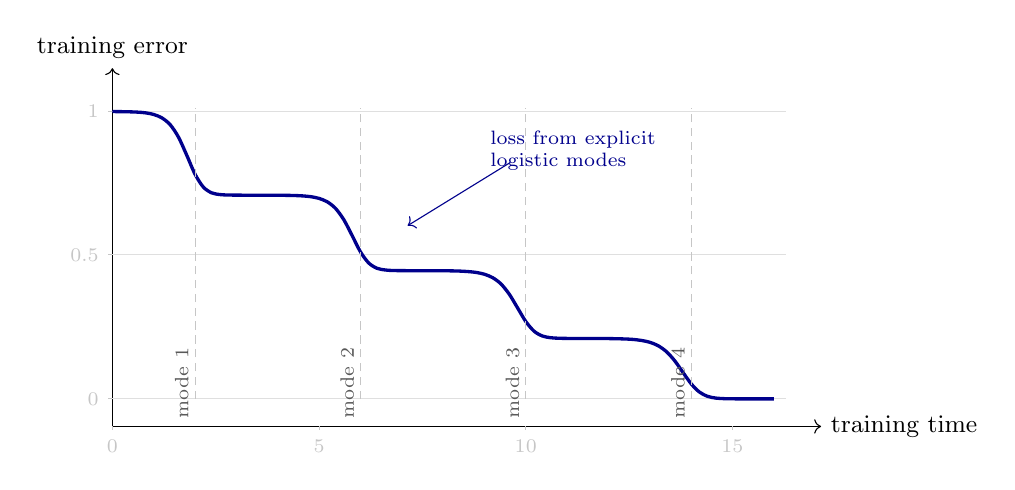
\begin{tikzpicture}[x=1cm,y=1cm]
  \draw[->] (0,0) -- (9,0) node[right] {\small training time};
  \draw[->] (0,0) -- (0,4.55) node[above] {\small training error};
  \foreach \x/\lab in {0/0,2.625/5,5.25/10,7.875/15} {
    \draw[gray!45] (\x,0) -- (\x,-0.05) node[below,font=\scriptsize] {\lab};
  }
  \foreach \y/\lab in {0.35/0,2.18/0.5,4.0/1} {
    \draw[gray!45] (0,\y) -- (-0.05,\y) node[left,font=\scriptsize] {\lab};
  }
  \draw[gray!25] (0,0.35) -- (8.55,0.35);
  \draw[gray!25] (0,2.18) -- (8.55,2.18);
  \draw[gray!25] (0,4.0) -- (8.55,4.0);
  \draw[blue!55!black,very thick,smooth] plot coordinates {
    (0.000,3.999) (0.105,3.998) (0.210,3.996) (0.315,3.992) (0.420,3.983)
    (0.525,3.962) (0.630,3.918) (0.735,3.831) (0.840,3.673) (0.945,3.443)
    (1.050,3.203) (1.155,3.040) (1.260,2.967) (1.365,2.945) (1.470,2.939)
    (1.575,2.938) (1.680,2.937) (1.785,2.937) (1.890,2.937) (1.995,2.937)
    (2.100,2.936) (2.205,2.935) (2.310,2.933) (2.415,2.928) (2.520,2.918)
    (2.625,2.896) (2.730,2.852) (2.835,2.768) (2.940,2.624) (3.045,2.424)
    (3.150,2.218) (3.255,2.076) (3.360,2.009) (3.465,1.987) (3.570,1.980)
    (3.675,1.979) (3.780,1.978) (3.885,1.978) (3.990,1.978) (4.095,1.978)
    (4.200,1.977) (4.305,1.976) (4.410,1.973) (4.515,1.967) (4.620,1.956)
    (4.725,1.933) (4.830,1.889) (4.935,1.810) (5.040,1.680) (5.145,1.507)
    (5.250,1.333) (5.355,1.210) (5.460,1.149) (5.565,1.127) (5.670,1.120)
    (5.775,1.118) (5.880,1.118) (5.985,1.118) (6.090,1.117) (6.195,1.117)
    (6.300,1.116) (6.405,1.114) (6.510,1.111) (6.615,1.105) (6.720,1.092)
    (6.825,1.069) (6.930,1.026) (7.035,0.951) (7.140,0.836) (7.245,0.688)
    (7.350,0.542) (7.455,0.437) (7.560,0.382) (7.665,0.360) (7.770,0.353)
    (7.875,0.351) (7.980,0.350) (8.085,0.350) (8.190,0.350) (8.295,0.350)
    (8.400,0.350)
  };
  \foreach \x/\name in {1.05/1,3.15/2,5.25/3,7.35/4} {
    \draw[gray!45,densely dashed] (\x,0.35) -- (\x,4.05);
    \node[font=\scriptsize,gray!70!black,rotate=90,anchor=south] at (\x+0.04,0.55) {mode \name};
  }
  \node[font=\scriptsize,align=left,blue!55!black] at (5.85,3.5)
    {loss from explicit\\logistic modes};
  \draw[->,blue!55!black] (5.05,3.35) -- (3.75,2.55);
\end{tikzpicture}
\caption{A learning staircase computed from the deep-linear solution of Saxe et al. In mode $i$, $s_i$ is the target singular value and $a_i(t)$ is the coefficient learned by time $t$, satisfying $\tau\dot a_i=2a_i(s_i-a_i)$. The curve plots normalized training error $\sum_i(s_i-a_i(t))^2$ for $\tau=0.5$ and $s=(1,0.95,0.9,0.85)$, with small initial coefficients chosen so the four modes turn on at separated times. Each mode turning on produces one drop.}
\label{fig:staircase}
\end{figure}

\begin{openproblem}[Opposing staircases]
Watanabe's theorem is Bayesian; gradient descent is not. (What bridging the two would mean for safety is discussed in~\cite{lehalleur2025}.) Build the bridge first in the deep-linear staircase above, where both sides are explicit. Each plateau sits at a saddle where only the $k$ largest modes have been learned, and there the definition itself is part of the problem: the local learning coefficient is defined at a local \emph{minimum}, as the volume exponent of the set of nearby parameters fitting almost as well, but a saddle has descent directions, so that volume does not shrink to zero. Formulate the right local invariant at the $k$th saddle (one candidate, the \emph{two-sided} exponent: the volume of nearby parameters whose loss lies within $\varepsilon$ of the saddle's, above or below, shrinks like $\varepsilon^{\lambda}$), compute it for the deep-linear network, and prove or refute the monotone picture that gives this problem its name: as gradient flow descends the staircase of losses, the invariant that controls generalization climbs an opposing staircase. As a first check, the estimator of Lau et al.~\cite{lau2023} runs at any parameter, saddle or not; run it along a simulated staircase and see.
\end{openproblem}

\subsection{Generalization beyond the training distribution}

The theory above concerns generalization \emph{in distribution}: test data drawn from the same law as the training data. The safety-critical regime is the opposite one, \emph{out of distribution}---how a trained system behaves on inputs unlike anything it saw in training---and there the gap between fitting and understanding reopens. Two parameter settings with identical training loss can implement different mechanisms (as above) and therefore extrapolate differently; which extrapolation gradient descent selects is, at present, something we observe after the fact rather than predict.

In \emph{goal misgeneralization}~\cite{langosco2022}, a system under \emph{distribution shift}---a deployment input distribution unlike the one it trained on---keeps its \emph{capabilities} while pursuing a \emph{different goal} from the one intended. The standard example is an agent trained to collect a coin in a video game where the coin always sat at the right end of the level: it learned ``move right,'' not ``reach the coin,'' and the two came apart the moment the coin moved. Capable but misdirected is the dangerous quadrant, and it is invisible to any testing that stays in distribution.

The pattern is old enough to have a name, \emph{Goodhart's law}: a proxy optimized hard enough stops tracking the goal it stood for. On the training levels, ``move right'' was a perfect proxy for ``reach the coin,'' so optimization could not tell them apart; the shift revealed which one the network had learned. Reward hacking (Section~\ref{sec:epistemics}) is the same law during training; goal misgeneralization is the law at deployment.

\begin{openproblem}[A predictive theory of out-of-distribution generalization]
In the coin-collecting environment of Langosco et al.~\cite{langosco2022}, reduced to one dimension, two policies fit the training data perfectly: ``move right'' (the proxy) and ``go to the coin'' (the intended goal), which agree whenever the coin sits at the right end. Train a two-layer network by gradient descent to imitate optimal play, randomizing the coin's position in an $\varepsilon$-fraction of training episodes. Determine the probability, over the random initialization, that the trained network follows the proxy on a probe state where the two policies disagree, as a function of $\varepsilon$, the width, and the input encoding. For linear policies the answer is a theorem---the encoding, not the initialization, decides---and the standard infinite-width limits follow it; for networks of finite width it is open at every $\varepsilon$, including $\varepsilon=0$, already at width two.
\end{openproblem}

% \noindent\emph{Entry points.} Algebraic geometry (resolution of singularities, log canonical thresholds), statistical mechanics, probability, dynamical systems, statistical learning theory.

%\input{sections-revised/control}       % parked: not in current compile
%\input{sections-revised/topology}      % parked: not in current compile
\section{Getting started in AI safety}
\label{sec:conclusion}

%Mathematicians do not need to become machine-learning engineers, and beautiful problems do not need safety justifications. But the profession already knows how to do something the world badly needs: turn vague pressure into definitions, invariants, examples, counterexamples, and theorems. The difficulty is choosing where that craft should go.

Technological progress is a human choice, not a law of nature. When mathematical ideas help build systems whose effects will be felt at civilizational scale, truth-seeking remains a core value, but it is no longer the only value in view. The civic mathematician also asks what our truths are for: whether they can help design AI systems to be more legible, more accountable, and easier to steer toward coexistence with us.

The open problems above are meant as entry points into the new field of Math for AI Safety. Other ways in are workshops like \href{https://www.iliadconference.com}{ILIAD}, the \href{https://www.arena.education/}{ARENA} curriculum, research programs like \href{https://www.matsprogram.org/}{MATS} and \href{https://sparai.org/}{SPAR}, and organizations like \href{https://humancompatible.ai/}{CHAI}, \href{https://constellation.org/}{Constellation}, \href{https://www.far.ai/}{FAR AI}, and \href{https://resolution.org}{Resolution}. Funding for work in this area is available from grantmakers like \href{https://coefficientgiving.org/funds/navigating-transformative-ai/}{Coefficient Giving}, \href{https://www.cooperativeai.com/}{CAIF}, \href{https://survivalandflourishing.fund/}{SFF}, and \href{https://alignmentproject.aisi.gov.uk/}{UK AISI}. % pass 2: resource list moved before the closing line so the section ends on the exhortation, not the link list
I hope you'll pick a problem whose language already feels like home, strip it down to the simplest interesting case, and start proving things!

\section*{Acknowledgments}

I thank Jesse Hoogland, Hyojeong Son, Jacob Tsimerman, Claude Fable 5, Claude Opus 4.8, and GPT 5.5 and 5.6 Sol for many inspiring conversations. Scott Aaronson, Ahmed Bou-Rabee, Vince Conitzer, Jonathan Gabor, Chris Hillar, Brad Knox, Phil Sosoe, Samuel Speas, Kate Stange, Steve Strogatz, Ariel Yadin, and an anonymous referee provided valuable feedback on an early draft.

\appendix

\section{A glossary for mathematicians}
\label{app:glossary}

\begin{longtable}{@{}p{0.26\textwidth} p{0.68\textwidth}@{}}
\glsentry{neural-network}{neural network} & a function with millions to billions of adjustable parameters (its \emph{weights}), built by composing simple layers and tuned by \emph{gradient descent} to reduce a training \emph{loss}. \\[5pt]
\glsentry{language-model}{language model} & a neural network trained to predict the next token of text; today's chat systems are language models further trained to follow instructions. \\[5pt]
\glsentry{token}{token} & the atomic unit (word or word-fragment) a language model reads and predicts. \\[5pt]
\glsentry{loss}{loss} & the scalar a network is trained to minimize; for language models, the negative log-probability it assigned to the actual next token. \\[5pt]
\glsentry{weights}{weights} & the trainable parameters of an artificial neural network: the entries of its matrices, trained by gradient descent and fixed at deployment time. \\[5pt]
\glsentry{activations}{activations} & the values that flow through the network on a given input (the outputs of its neurons and layers), as opposed to the fixed weights. \\[5pt]
\glsentry{activation-space}{activation space} & the copy of $\mathbb{R}^n$ in which a given layer's activations live, one coordinate per neuron; feature directions are directions in this space. \\[5pt]
\glsentry{gradient-descent}{gradient descent} & the optimizer: repeatedly nudge the parameters $w$ against the gradient of the loss, $w \leftarrow w - \eta\,\nabla L(w)$. \\[5pt]
\glsentry{relu}{ReLU} & the rectified linear unit $x \mapsto \max(0,x)$, a canonical piecewise-linear nonlinearity; modern transformers often use smooth or gated variants instead (GELU, SiLU, SwiGLU). \\[5pt]
\glsentry{transformer}{transformer} & the dominant network architecture for language: a stack of layers that mix information across token positions by \emph{attention} (each position selectively reads from the others) and read from / write to the residual stream. \\[5pt]
\glsentry{residual-stream}{residual stream} & the running vector of activations a transformer reads from and writes to at each layer; a natural home for feature directions. \\[5pt]
\glsentry{feature}{feature} & a hypothesized variable or property a network represents in its activations (e.g.\ ``the text is in French''). \\[5pt]
\glsentry{probe}{probe} & a simple (usually linear) function of a network's activations, trained or searched to read off some quantity of interest. \\[5pt]
\glsentry{policy}{policy} & an agent's rule for choosing actions from states (a possibly randomized map from states to actions). \\[5pt]
\glsentry{reward-hacking}{reward hacking} & raising a measured reward signal in ways that defeat the intent behind it; Goodhart's law as it appears in agents trained by reward. \\[5pt]
\glsentry{superposition}{superposition} & a hypothesized representation scheme in which a network stores more features than it has dimensions, as non-orthogonal directions, tolerable when few features are active at once. \\[5pt]
\glsentry{sparse-autoencoder}{sparse autoencoder} & a network trained to reconstruct another network's activations as sparse combinations of learned dictionary directions; an empirical tool for extracting features. \\[5pt]
\glsentry{interpretability}{interpretability} & reverse-engineering a trained network into human-understandable structure (circuits, features, algorithms), validated by intervention and not by human-readable description alone. \\[5pt]
% corrigibility row commented out 2026-07-09: its first use (the intro's control/coexistence footnote) is commented out; restore both together.
% \glsentry{corrigibility}{corrigibility} & the property that an AI system accepts correction, modification, and shutdown by its human principals, rather than resisting them. \\[5pt]
\glsentry{gradual-disempowerment}{gradual disempowerment} & the risk that humans lose influence over the institutions that shape their lives, by incremental delegation to AI systems we do not understand rather than by any sudden takeover. \\
\end{longtable}

\begin{thebibliography}{99}

% 2026-07-12: eleven uncited entries deleted outright per the citation review
% (edits/citation-recommendations.md), along with einsteinarena and sanborn2022
% (cut with their citations). Restored the same day with new one-sentence homes:
% rao1999, wald1950, wentworth2025, ngo2025scale.

\bibitem{abbe2023} Abbe, E., Boix-Adser\`a, E., and Misiakiewicz, T. (2023). SGD learning on neural networks: leap complexity and saddle-to-saddle dynamics. \emph{Conference on Learning Theory (COLT)} 2023. \arxiv{2302.11055}.

\bibitem{aharon2006} Aharon, M., Elad, M., and Bruckstein, A. M. (2006). On the uniqueness of overcomplete dictionaries, and a practical way to retrieve them. \emph{Linear Algebra and its Applications} 416(1), 48--67.

\bibitem{alon2026remarks} Alon, N., Bloom, T. F., Gowers, W. T., Litt, D., Sawin, W., Shankar, A., Tsimerman, J., Wang, V., and Wood, M. M. (2026). Remarks on the disproof of the unit distance conjecture. \arxiv{2605.20695}.

\bibitem{alquier2020} Alquier, P., and Ridgway, J. (2020). Concentration of tempered posteriors and of their variational approximations. \emph{Annals of Statistics} 48(3), 1475--1497. \arxiv{1706.09293}.

\bibitem{arditi2024} Arditi, A., Obeso, O., Syed, A., Paleka, D., Panickssery, N., Gurnee, W., and Nanda, N. (2024). Refusal in language models is mediated by a single direction. \emph{Advances in Neural Information Processing Systems} 37. \arxiv{2406.11717}.


\bibitem{barasz2014} Bar\'asz, M., Christiano, P., Fallenstein, B., Herreshoff, M., LaVictoire, P., and Yudkowsky, E. (2014). Robust cooperation in the Prisoner's Dilemma: program equilibrium via provability logic. \arxiv{1401.5577}.


\bibitem{bricken2023} Bricken, T., et al. (2023). Towards monosemanticity: decomposing language models with dictionary learning. \emph{Transformer Circuits Thread}, Anthropic. \url{https://transformer-circuits.pub/2023/monosemantic-features}.



\bibitem{caizhang2014} Cai, T. T., and Zhang, A. (2014). Sparse representation of a polytope and recovery of sparse signals and low-rank matrices. \emph{IEEE Transactions on Information Theory} 60(1), 122--132. \arxiv{1306.1154}.

\bibitem{candes2006} Cand\`es, E. J., Romberg, J., and Tao, T. (2006). Robust uncertainty principles: exact signal reconstruction from highly incomplete frequency information. \emph{IEEE Transactions on Information Theory} 52(2), 489--509.

\bibitem{candes2008} Cand\`es, E. J. (2008). The restricted isometry property and its implications for compressed sensing. \emph{Comptes Rendus Math\'ematique} 346(9--10), 589--592.




\bibitem{chughtai2023} Chughtai, B., Chan, L., and Nanda, N. (2023). A toy model of universality: reverse-engineering how networks learn group operations. \emph{International Conference on Machine Learning} 2023. \arxiv{2302.03025}.

\bibitem{cooper2025} Cooper, E., Oesterheld, C., and Conitzer, V. (2025). Characterising simulation-based program equilibria. \emph{Proceedings of AAAI} 2025. \arxiv{2412.14570}.

\bibitem{critch2016} Critch, A. (2019). A parametric, resource-bounded generalization of L\"ob's theorem, and a robust cooperation criterion for open-source game theory. \emph{The Journal of Symbolic Logic} 84(4), 1368--1381. \arxiv{1602.04184}.

\bibitem{critch2022} Critch, A., Dennis, M., and Russell, S. (2022). Cooperative and uncooperative institution designs: surprises and problems in open-source game theory. \arxiv{2208.07006}.

\bibitem{cunningham2023} Cunningham, H., Ewart, A., Riggs, L., Huben, R., and Sharkey, L. (2023). Sparse autoencoders find highly interpretable features in language models. \arxiv{2309.08600}.


\bibitem{donoho2006} Donoho, D. L. (2006). Compressed sensing. \emph{IEEE Transactions on Information Theory} 52(4), 1289--1306.

\bibitem{dyson2009} Dyson, F. (2009). Birds and frogs. \emph{Notices of the American Mathematical Society} 56(2), 212--223.



\bibitem{eisenstat2025} Eisenstat, S. (2025). Condensation: a theory of concepts. Manuscript. \url{https://www.sameisenstat.net/doc/condensation-25-07.pdf}.

\bibitem{elhage2022} Elhage, N., et al. (2022). Toy models of superposition. \emph{Transformer Circuits Thread}. \arxiv{2209.10652}.





\bibitem{garfinkle2019} Garfinkle, C. J., and Hillar, C. J. (2019). On the uniqueness and stability of dictionaries for sparse representation of noisy signals. \emph{IEEE Transactions on Signal Processing} 67(23), 5884--5892. \arxiv{1606.06997}.

\bibitem{garrabrant2016} Garrabrant, S., Benson-Tilsen, T., Critch, A., Soares, N., and Taylor, J. (2016). Logical induction. \arxiv{1609.03543}.

\bibitem{gowers2000} Gowers, W. T. (2000). The two cultures of mathematics. In \emph{Mathematics: Frontiers and Perspectives} (V. Arnold, M. Atiyah, P. Lax, and B. Mazur, eds.), American Mathematical Society, 65--78.

\bibitem{gribonval2015} Gribonval, R., Jenatton, R., and Bach, F. (2015). Sparse and spurious: dictionary learning with noise and outliers. \emph{IEEE Transactions on Information Theory} 61(11), 6298--6319. \arxiv{1407.5155}.

\bibitem{grunwald2012} Gr\"unwald, P. (2012). The safe Bayesian: learning the learning rate via the mixability gap. \emph{Algorithmic Learning Theory (ALT)} 2012, 169--183.





% 2026-07-13: entry moved here (was filed under its citation key "spherepacking2026",
% stranding Hariharan et al. between Sharkey and Tennenholtz).
\bibitem{spherepacking2026} Hariharan, S., Birkbeck, C., Lee, S., Ma, H. K. G., Mehta, B., Poiroux, A., and Viazovska, M. (2026). Progress in formalizing sphere packing in dimension~8. \arxiv{2604.23468}.

\bibitem{hillar2015} Hillar, C. J., and Sommer, F. T. (2015). When can dictionary learning uniquely recover sparse data from subsamples? \emph{IEEE Transactions on Information Theory} 61(11), 6290--6297. \arxiv{1106.3616}.

\bibitem{hironaka1964} Hironaka, H. (1964). Resolution of singularities of an algebraic variety over a field of characteristic zero. \emph{Annals of Mathematics} 79(1), 109--203; 79(2), 205--326.

\bibitem{howard1988} Howard, J. V. (1988). Cooperation in the Prisoner's Dilemma. \emph{Theory and Decision} 24(3), 203--213.



\bibitem{johnson1984} Johnson, W. B., and Lindenstrauss, J. (1984). Extensions of Lipschitz mappings into a Hilbert space. \emph{Contemporary Mathematics} 26, 189--206.

\bibitem{khan2023} Khan, M. E., and Rue, H. (2023). The Bayesian learning rule. \emph{Journal of Machine Learning Research} 24(281), 1--46. \arxiv{2107.04562}.

\bibitem{kulveit2025} Kulveit, J., Douglas, R., Ammann, N., Turan, D., Krueger, D., and Duvenaud, D. (2025). Gradual disempowerment: systemic existential risks from incremental AI development. \arxiv{2501.16946}.






\bibitem{kwa2025} Kwa, T., West, B., Becker, J., et al. (2025). Measuring AI ability to complete long software tasks. METR report; \emph{Advances in Neural Information Processing Systems} 38. \arxiv{2503.14499}.

% 2026-07-13: Orseau dropped to match the published ICML author list (he appears
% only on the arXiv version); first author kept as "Langosco" per Lionel.
\bibitem{langosco2022} Langosco, L., Koch, J., Sharkey, L., Pfau, J., and Krueger, D. (2022). Goal misgeneralization in deep reinforcement learning. \emph{International Conference on Machine Learning} 2022. \arxiv{2105.14111}.

\bibitem{lau2023} Lau, E., Furman, Z., Wang, G., Murfet, D., and Wei, S. (2025). The local learning coefficient: a singularity-aware complexity measure. \emph{Artificial Intelligence and Statistics (AISTATS)} 2025. \arxiv{2308.12108}.


\bibitem{lob1955} L\"ob, M. H. (1955). Solution of a problem of Leon Henkin. \emph{The Journal of Symbolic Logic} 20(2), 115--118.



\bibitem{marchetti2024} Marchetti, G. L., Hillar, C., Kragic, D., and Sanborn, S. (2024). Harmonics of learning: universal Fourier features emerge in invariant networks. \emph{Conference on Learning Theory (COLT)} 2024. \arxiv{2312.08550}.

\bibitem{mathlib2020} The mathlib Community. (2020). The Lean mathematical library. \emph{Certified Programs and Proofs (CPP)} 2020, 367--381. \arxiv{1910.09336}.

\bibitem{murfet2026} Murfet, D., Gordon, A., Adam, M., Wang, G., Hoogland, J., Baker, G., Snell, W., van Wingerden, S., Newgas, A., Snikkers, B., and Hitchcock, R. (2026). Spectroscopy at scale: finding interpretable structure in Pythia-1.4B. Timaeus, research report. \url{https://timaeus.co/research/2026-04-21-spectroscopy-main/}.

\bibitem{nanda2023} Nanda, N., Chan, L., Lieberum, T., Smith, J., and Steinhardt, J. (2023). Progress measures for grokking via mechanistic interpretability. \emph{International Conference on Learning Representations} 2023. \arxiv{2301.05217}.

\bibitem{ngo2025scale} Ngo, R. (2025). Towards a scale-free theory of intelligent agency. LessWrong essay. \url{https://www.lesswrong.com/posts/5tYTKX4pNpiG4vzYg/towards-a-scale-free-theory-of-intelligent-agency}.

\bibitem{oesterheld2021} Oesterheld, C., and Conitzer, V. (2021). Safe Pareto improvements for delegated game playing. \emph{International Conference on Autonomous Agents and Multiagent Systems (AAMAS)} 2021; journal version, \emph{Autonomous Agents and Multi-Agent Systems} 36 (2022).

\bibitem{openai2026unitdistance} OpenAI. (2026). An OpenAI model has disproved a central conjecture in discrete geometry. \url{https://openai.com/index/model-disproves-discrete-geometry-conjecture/}.

\bibitem{park2023} Park, K., Choe, Y. J., and Veitch, V. (2024). The linear representation hypothesis and the geometry of large language models. \emph{International Conference on Machine Learning} 2024. \arxiv{2311.03658}.

\bibitem{parr2022} Parr, T., Pezzulo, G., and Friston, K. J. (2022). \emph{Active Inference: The Free Energy Principle in Mind, Brain, and Behavior}. MIT Press.

\bibitem{pearl2009} Pearl, J. (2009). \emph{Causality: Models, Reasoning, and Inference}, 2nd ed. Cambridge University Press.

\bibitem{lehalleur2025} Pepin Lehalleur, S., Hoogland, J., Farrugia-Roberts, M., Wei, S., Gietelink Oldenziel, A., Wang, G., Carroll, L., and Murfet, D. (2025). You are what you eat: AI alignment requires understanding how data shapes structure and generalisation. \arxiv{2502.05475}.

\bibitem{rao1999} Rao, R. P. N., and Ballard, D. H. (1999). Predictive coding in the visual cortex: a functional interpretation of some extra-classical receptive-field effects. \emph{Nature Neuroscience} 2(1), 79--87.


\bibitem{richens2024} Richens, J., and Everitt, T. (2024). Robust agents learn causal world models. \emph{International Conference on Learning Representations} 2024. \arxiv{2402.10877}.


\bibitem{richens2025general} Richens, J., Everitt, T., and Abel, D. (2025). General agents need world models. \emph{International Conference on Machine Learning} 2025. \arxiv{2506.01622}.

\bibitem{saff1997} Saff, E. B., and Kuijlaars, A. B. J. (1997). Distributing many points on a sphere. \emph{The Mathematical Intelligencer} 19(1), 5--11.


\bibitem{sawin2026} Sawin, W. (2026). An explicit lower bound for the unit distance problem. \arxiv{2605.20579}.

\bibitem{saxe2014} Saxe, A. M., McClelland, J. L., and Ganguli, S. (2014). Exact solutions to the nonlinear dynamics of learning in deep linear neural networks. \emph{International Conference on Learning Representations} 2014. \arxiv{1312.6120}.

\bibitem{schelling1960} Schelling, T. C. (1960). \emph{The Strategy of Conflict}. Harvard University Press.

\bibitem{sharkey2025} Sharkey, L., et al. (2025). Open problems in mechanistic interpretability. \emph{Transactions on Machine Learning Research} 2025. \arxiv{2501.16496}.






\bibitem{tennenholtz2004} Tennenholtz, M. (2004). Program equilibrium. \emph{Games and Economic Behavior} 49(2), 363--373.


\bibitem{thurston1994} Thurston, W. P. (1994). On proof and progress in mathematics. \emph{Bulletin of the American Mathematical Society} 30(2), 161--177. \arxiv{math/9404236}.


% 2026-07-13: entry moved here (von Neumann under V; it sat between OpenAI and Park).
\bibitem{vnm1944} von Neumann, J., and Morgenstern, O. (1944). \emph{Theory of Games and Economic Behavior}. Princeton University Press.

\bibitem{wald1950} Wald, A. (1950). \emph{Statistical Decision Functions}. Wiley.

\bibitem{watanabe2009} Watanabe, S. (2009). \emph{Algebraic Geometry and Statistical Learning Theory}. Cambridge University Press.

\bibitem{watanabe2013} Watanabe, S. (2013). A widely applicable Bayesian information criterion. \emph{Journal of Machine Learning Research} 14, 867--897.

\bibitem{wentworth2025} Wentworth, J., and Lorell, D. (2025). Natural latents: latent variables stable across ontologies. \arxiv{2509.03780}.

\bibitem{zhang2017} Zhang, C., Bengio, S., Hardt, M., Recht, B., and Vinyals, O. (2017). Understanding deep learning requires rethinking generalization. \emph{International Conference on Learning Representations} 2017. \arxiv{1611.03530}.


\end{thebibliography}


\end{document}
